% Build: latexmk -xelatex slides.tex   (or: make slides)
\documentclass[aspectratio=169,11pt]{beamer}
\beamertemplatenavigationsymbolsempty
\setbeamertemplate{footline}[frame number]
\usepackage[no-math]{fontspec}
\setsansfont{DejaVu Sans}
\setmainfont{DejaVu Serif}
\setmonofont{DejaVu Sans Mono}[Scale=0.9]
\usepackage{polyglossia}
\setdefaultlanguage{russian}
\setotherlanguage{english}
\newfontfamily\cyrillicfontsf{DejaVu Sans}
\newfontfamily\cyrillicfont{DejaVu Serif}
\newfontfamily\cyrillicfonttt{DejaVu Sans Mono}[Scale=0.9]
\usepackage{amsmath,amssymb,booktabs}
\graphicspath{{../figures/}}
\setbeamerfont{frametitle}{size=\large}
\setbeamercolor{frametitle}{fg=blue!60!black}
\newcommand{\T}{^{\mathsf T}}

\title{RLC-цепь: модель ОДУ в частотной области}
\subtitle{Лабораторная работа 1, тема 6}
\date{2026}

\begin{document}

\begin{frame}
  \titlepage
  \centering\small Учебная модель против журнальной (дробной) на трёх физических объектах
\end{frame}

\begin{frame}{Задача и гипотезы}
  \textbf{Вопрос:} хватает ли учебной RLC-модели с идеальными элементами, или данные требуют дробных $L^{\beta}C^{\alpha}$?
  \medskip
  \begin{itemize}
    \item \textbf{H1.} Цепь из дискретных компонентов: учебная модель достаточна, $\alpha\approx1$.
    \item \textbf{H2.} Li-ion элемент: учебная RC-модель ошибается систематически, CPE~--- на порядок точнее; параметры дрейфуют со старением.
    \item \textbf{H3.} Моды резонатора: по одной моде модели неразличимы, но CPE предсказывает \emph{не зависящую от частоты} добротность.
  \end{itemize}
  \medskip
  \textbf{Данные (HTTP, закреплённые коммиты, SHA-256):}
  \begin{itemize}\small
    \item Zhang et al., \emph{Nature Commun.} 11, 1706 (2020): 299 спектров EIS за 598 циклов;
    \item impedance.py (JOSS 2020): 3 физические цепи $\times$ 2 повтора, 1~Гц--300~кГц;
    \item scikit-rf (IEEE MW Mag. 2022): полосковые резонаторы 36/72/144 мм, 1--5~ГГц.
  \end{itemize}
\end{frame}

\begin{frame}{Модели}
  \textbf{Учебная (T):}
  \[
    L\ddot q+R\dot q+\frac{q}{C}=v(t)\ \xrightarrow{\ \mathcal L,\ q(0)=\dot q(0)=0\ }\ Z_T(s)=R+sL+\frac{1}{sC}.
  \]
  \textbf{Журнальная (J)} — Westerlund \& Ekstam 1994, Radwan \& Salama 2011, Wang et al.\ \emph{Nat.\ Rev.\ Methods Primers} 2021:
  \[
    L\,D^{\beta}i+R\,i+\frac1Q D^{-\alpha}i=v(t),\qquad Z_J(s)=R+Ls^{\beta}+\frac{1}{Qs^{\alpha}}.
  \]
  \textbf{Утверждения} (доказаны в ноутбуке, допущения явные):
  \begin{enumerate}\small
    \item $Z_J|_{\alpha=\beta=1}=Z_T$ (вложенность);\quad
          $\alpha,\beta\le1\Rightarrow\operatorname{Re}Z\ge0$ для любой сети (пассивность);
    \item единственный резонанс $\omega_r=\bigl[\sin\frac{\alpha\pi}{2}/(QL\sin\frac{\beta\pi}{2})\bigr]^{1/(\alpha+\beta)}$;
    \item CPE: $\tan\delta=\cot(\alpha\pi/2)$ не зависит от $\omega$;
    \item мода линии: $Q_n\propto\omega_n/\alpha_{\rm att}(\omega_n)$ $\Rightarrow$ наклон $d\ln Q/d\ln f=1,\ \tfrac12,\ 0$ для $R=$const, скин-эффекта, CPE.
  \end{enumerate}
\end{frame}

\begin{frame}{Граф суперпозиции и матрица связей}
  \centering
  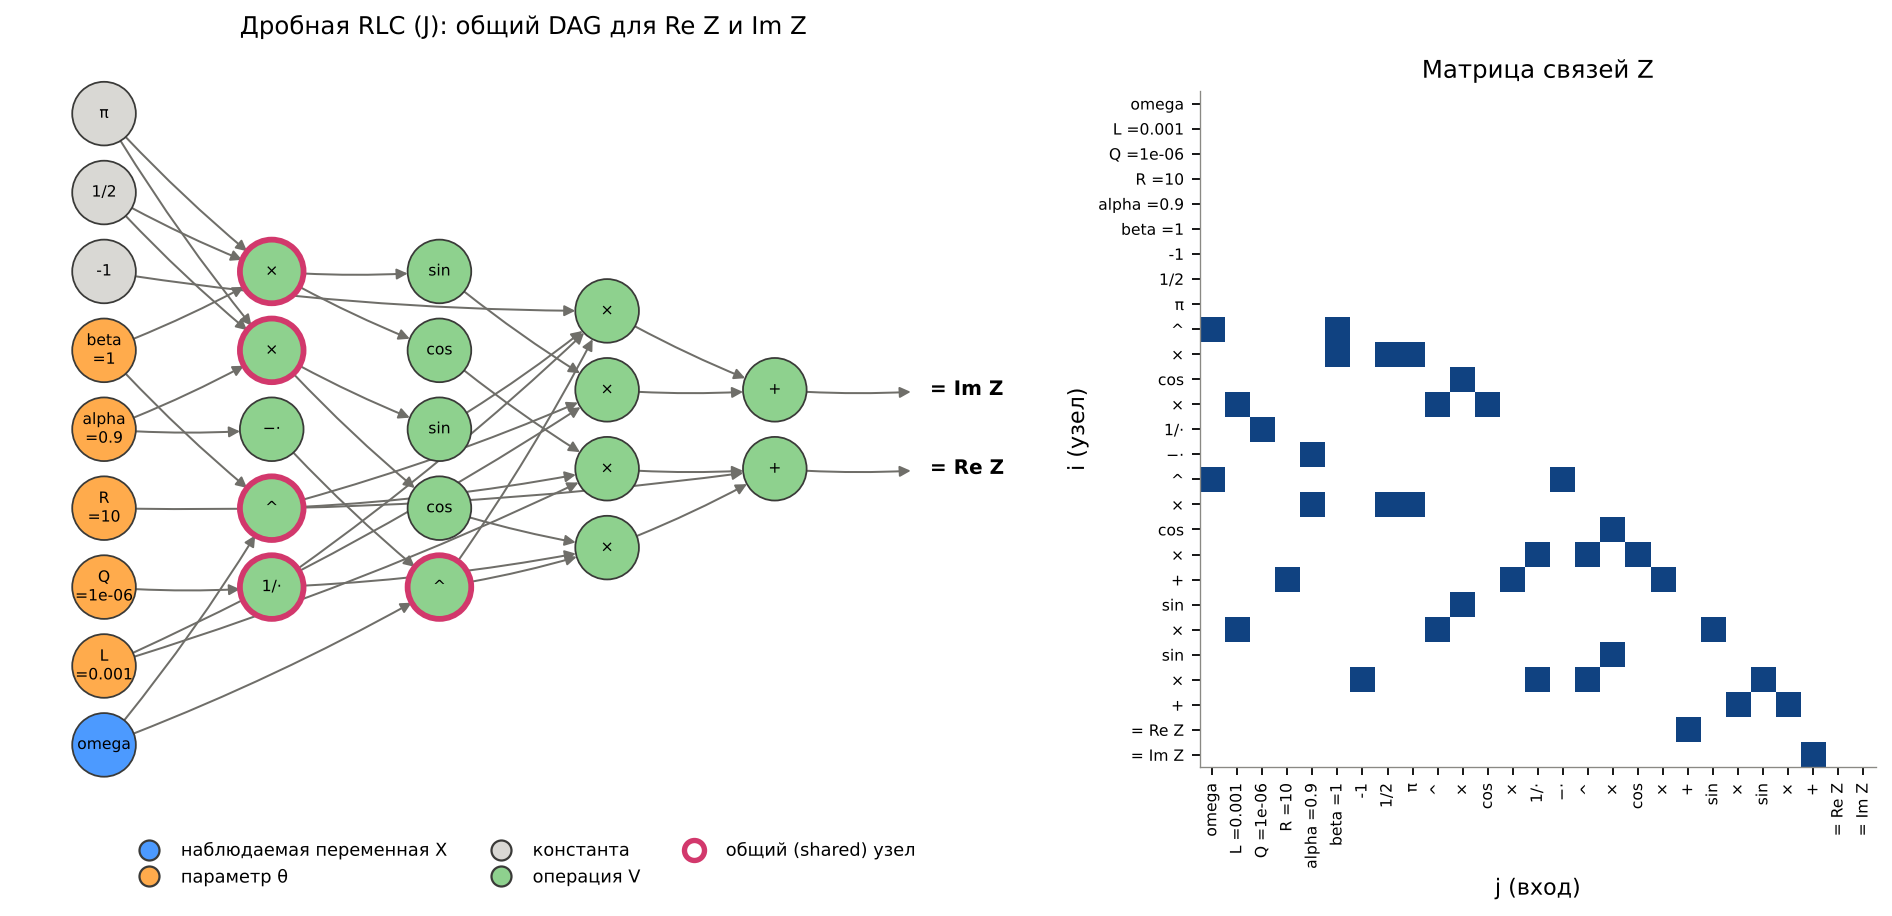
\includegraphics[width=0.9\linewidth]{dag_ZJ.png}\\[-1mm]
  \small DAG $(\operatorname{Re}Z_J,\operatorname{Im}Z_J)$: узлы $X$ (синие), $\theta$ (оранжевые), операции $V$; общие подграфы обведены.
  Словарь, позиционная матрица $Z$ и \texttt{networkx} восстанавливают выражения точно.
\end{frame}

\begin{frame}{Представления одной модели}
  \begin{columns}[T]
    \column{0.5\linewidth}
    \small
    \begin{itemize}
      \item строка грамматики \texttt{R0-L0-p(R1,Q1)};
      \item дерево разбора (series/parallel);
      \item выражение SymPy $\Rightarrow$ символьный якобиан;
      \item граф цепи + узловой анализ $Y=A\,\mathrm{diag}(y)A\T$~--- тот же $Z(s)$;
      \item передаточная функция (только целый порядок);
      \item DAG / словарь / матрица связей.
    \end{itemize}
    \column{0.5\linewidth}
    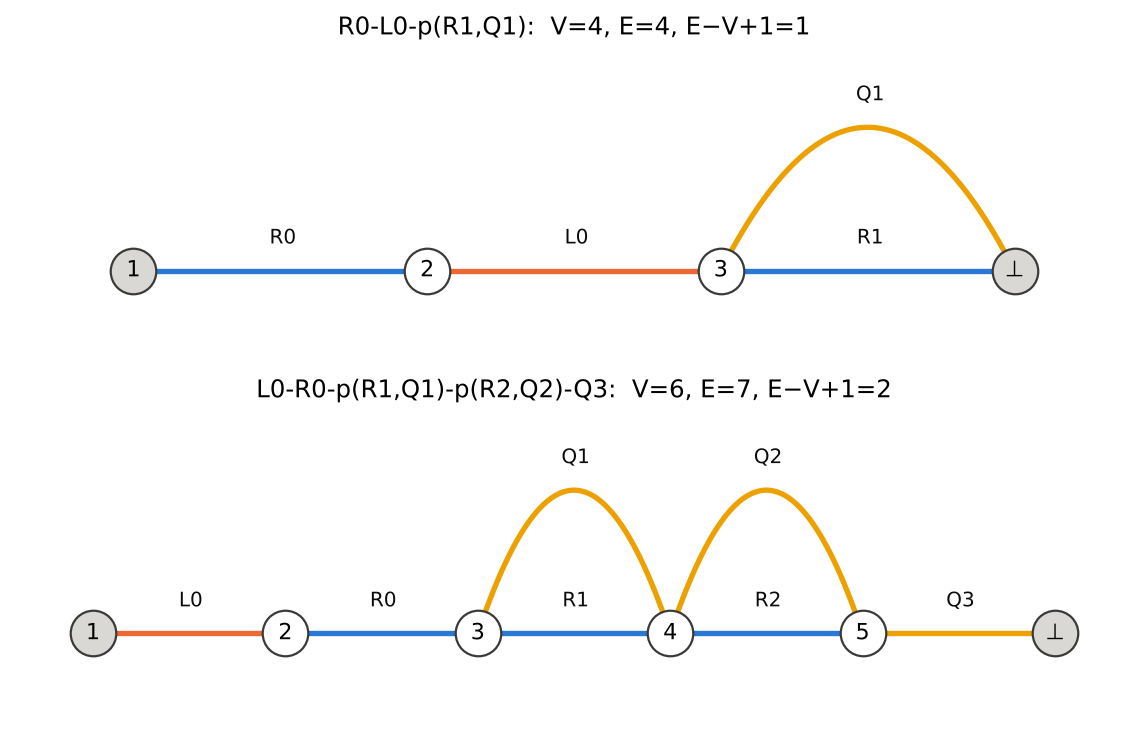
\includegraphics[width=\linewidth]{circuit_graphs.png}\\
    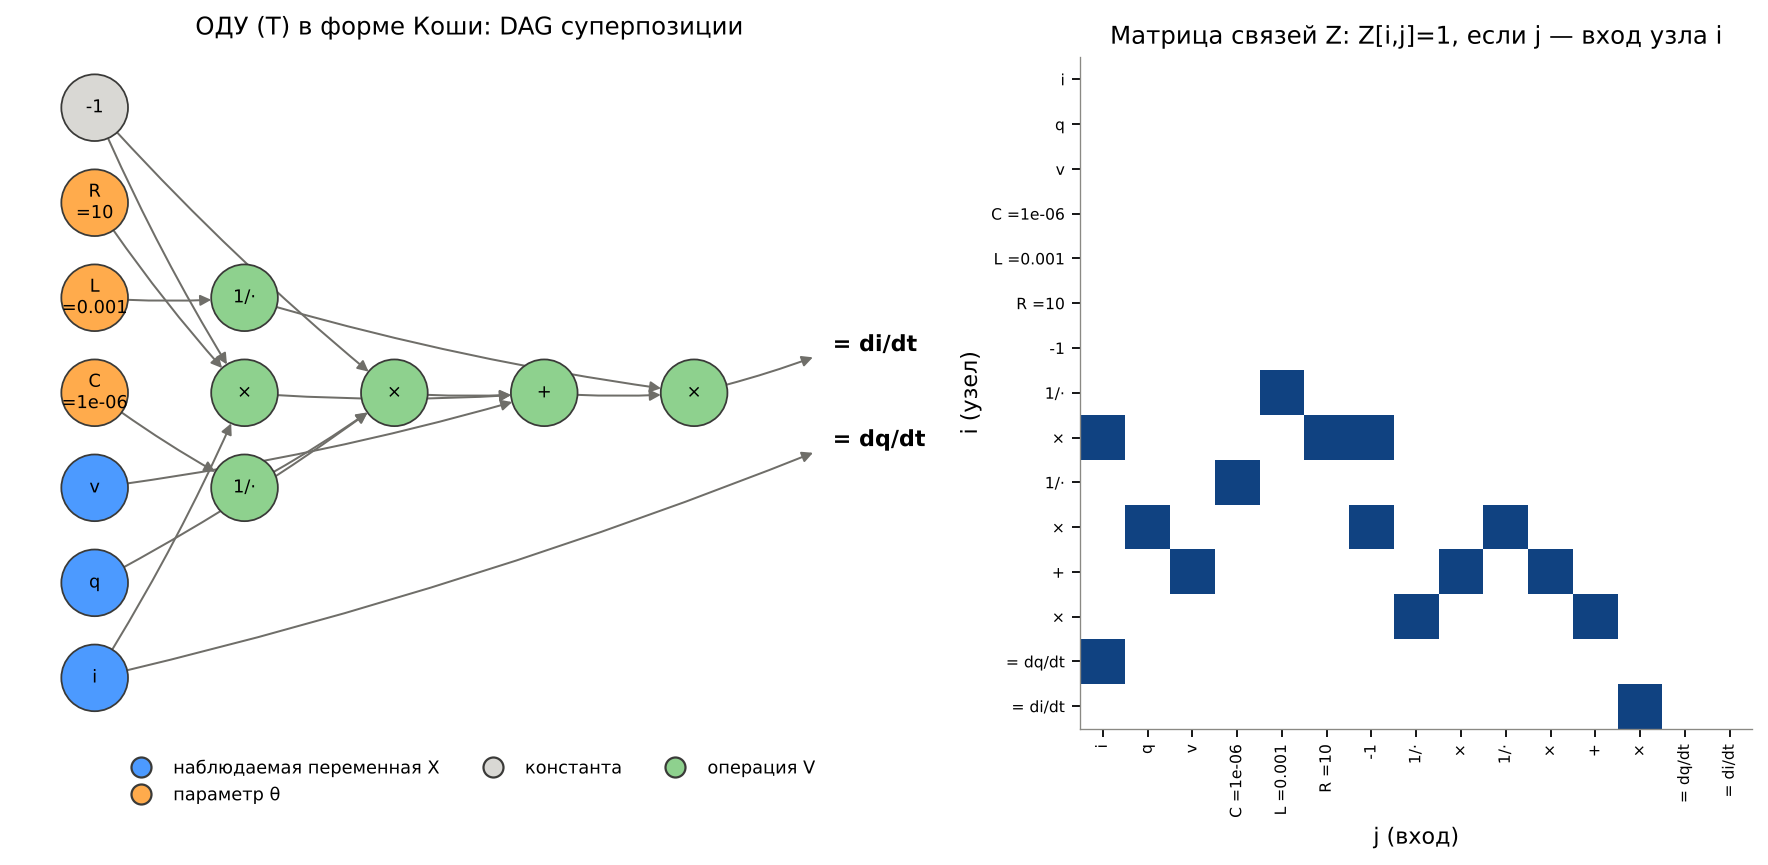
\includegraphics[width=\linewidth]{dag_ode.png}
  \end{columns}
\end{frame}

\begin{frame}{Векторное поле $\mathbb R^3\to\mathbb R^3$}
  \begin{columns}[T]
    \column{0.42\linewidth}
    \small
    Вынужденная цепь как автономное поле на $(x,y,\varphi)$:
    \[F=(y,\,-x-2\zeta y+u\cos\varphi,\,\Omega).\]
    \vspace{-3mm}
    \begin{itemize}
      \item $\operatorname{div}F=-2\zeta$ (диссипация),
      \item $\operatorname{rot}F=(u\sin\varphi,0,-2)$,
      \item $F\cdot\nabla H=-2\zeta y^2+uy\cos\varphi$ (баланс мощностей),
      \item Лиувилль: $\det D\Phi_\tau=e^{-2\zeta\tau}$ (проверено до $10^{-10}$).
    \end{itemize}
    \column{0.58\linewidth}
    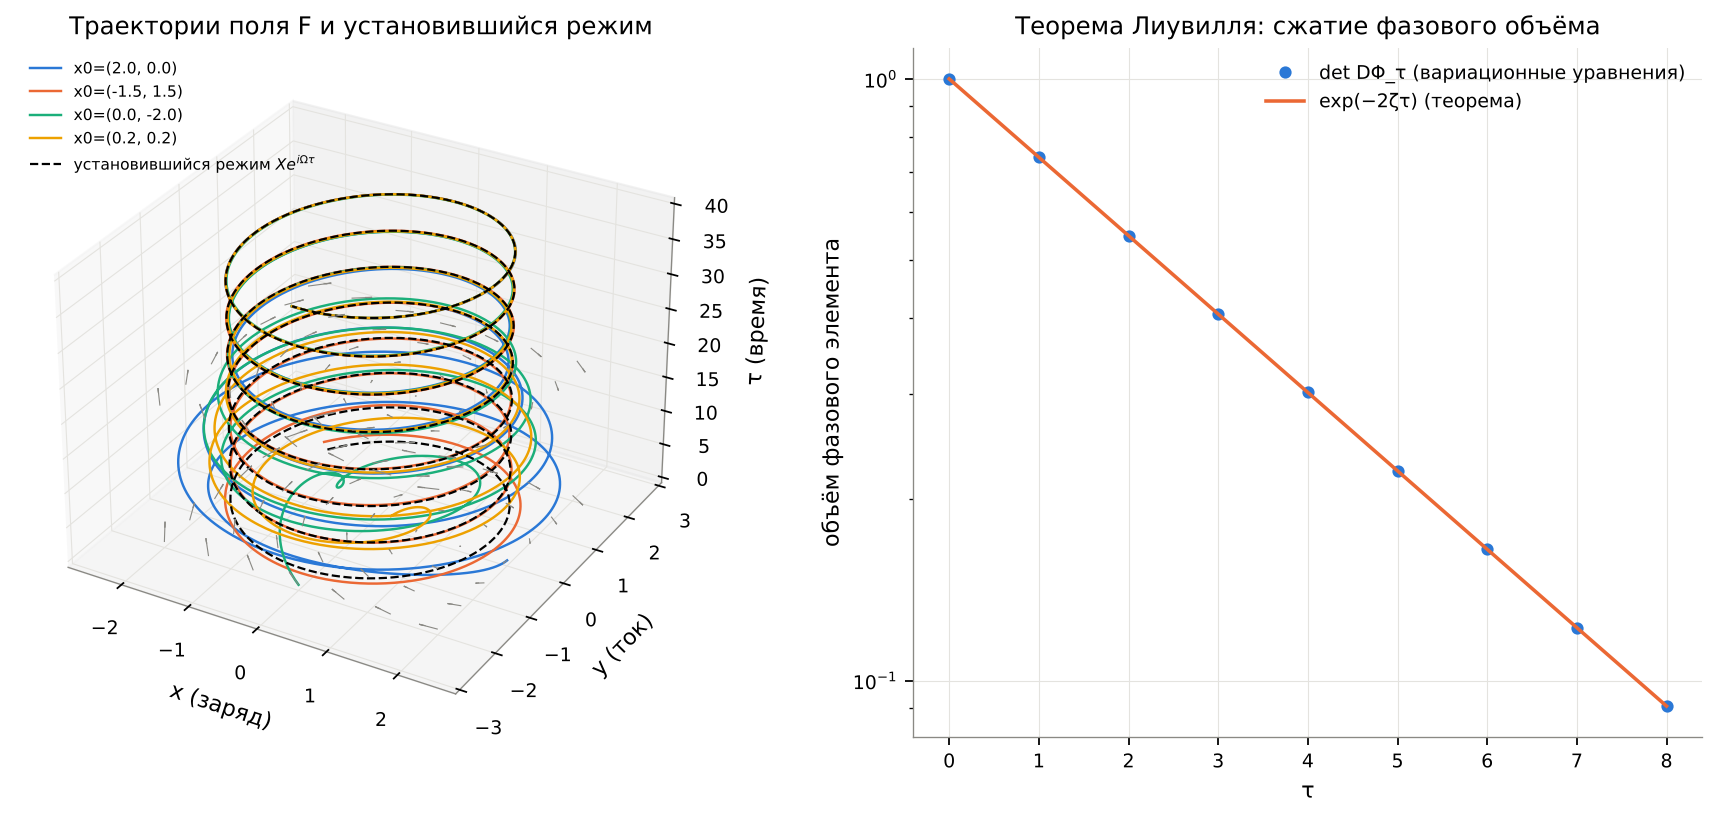
\includegraphics[width=\linewidth]{vector_field_3d.png}
  \end{columns}
\end{frame}

\begin{frame}{Данные в 3D с учётом времени}
  \centering
  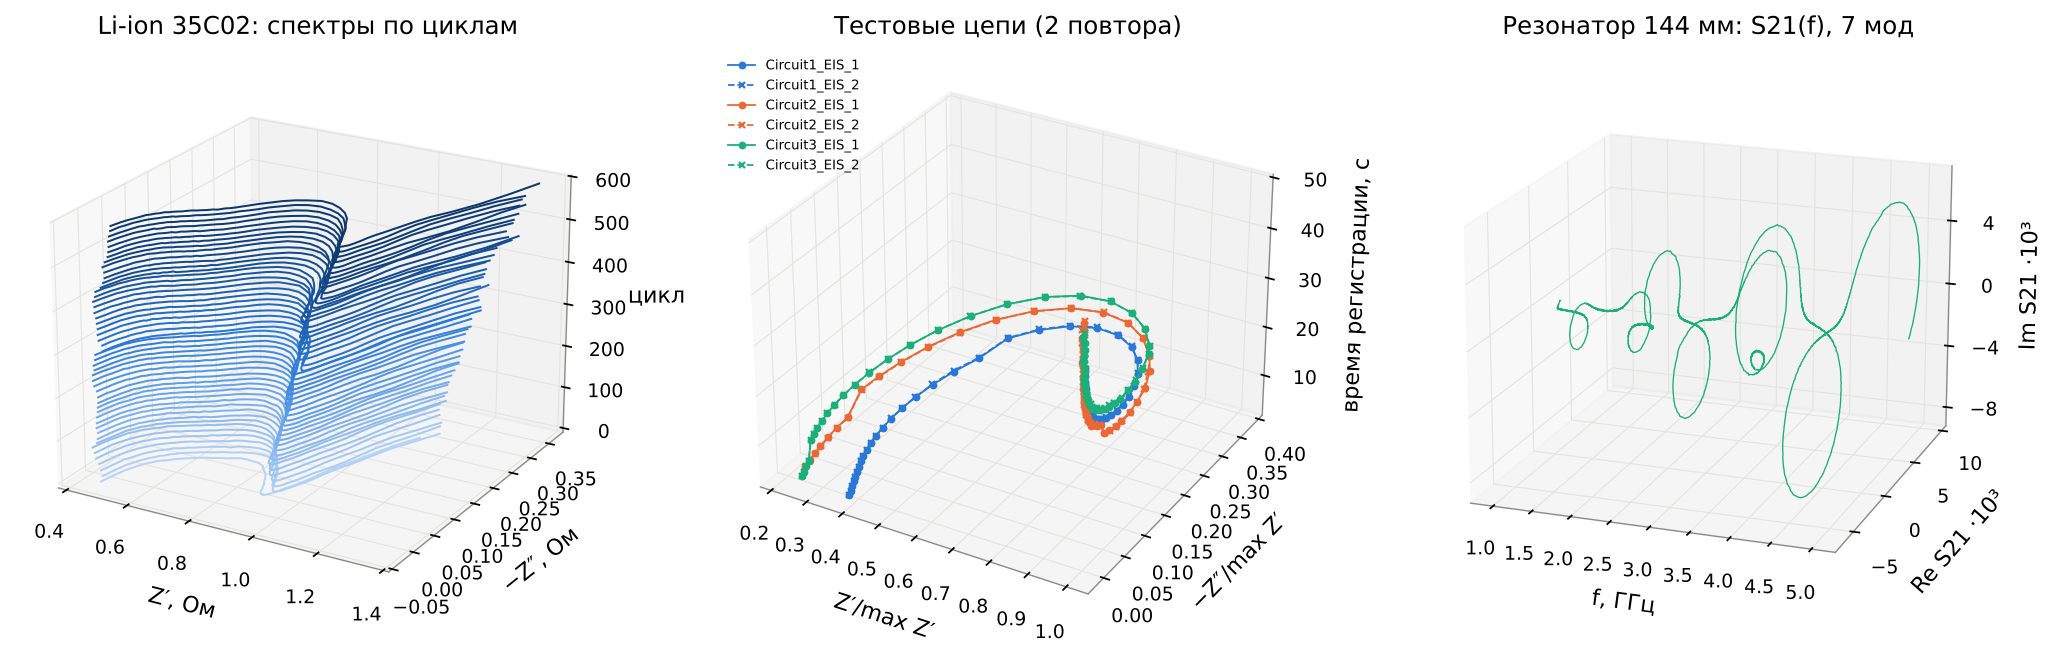
\includegraphics[width=\linewidth]{data_3d.png}\\
  \small Старение (циклы), время регистрации прибором, частота развёртки VNA.
\end{frame}

\begin{frame}{Оптимизатор и солвер}
  \begin{columns}[T]
    \column{0.48\linewidth}
    \footnotesize
    \textbf{Ошибка:} $S(\theta)=\sum_k|\hat Z_k(\theta)-Z_k|^2/|Z_k|^2$ (МНК = МП при шуме $\propto|Z|$); $\operatorname{Cov}\hat\theta\approx\hat\sigma^2(J\T J)^{+}$.
    \medskip

    Li-ion, модель J (10 параметров):\\[1mm]
    \begin{tabular}{lrr}\toprule
      метод & вычислений & с\\\midrule
      TRF (симв. якобиан) & 34 & 0{,}04\\
      LM (MINPACK) & 35 & 0{,}01\\
      multistart TRF & 2\,904 & 1{,}9\\
      CMA-ES + TRF & 15\,484 & 3{,}7\\
      DE + TRF & 102\,684 & 15\\\bottomrule
    \end{tabular}\\[1mm]
    все приходят в один минимум.
    \column{0.48\linewidth}
    \footnotesize
    \textbf{Солверы} (скачок напряжения, точное решение):\\[1mm]
    \begin{tabular}{lr}\toprule
      солвер & max ошибка, А\\\midrule
      RK45 / DOP853 & $5\cdot10^{-10}$\\
      Radau & $3\cdot10^{-11}$\\
      LSODA & $7\cdot10^{-9}$\\
      GL, $N=16\,001$, $O(h)$ & $1{,}4\cdot10^{-4}$\\
      Талбот (mpmath) & $2\cdot10^{-13}$\\\bottomrule
    \end{tabular}\\[1mm]
    Выбор: LSODA (жёсткие задачи), GL и Талбот для дробного порядка.
  \end{columns}
\end{frame}

\begin{frame}{Физические цепи: H1 в слабой форме}
  \centering
  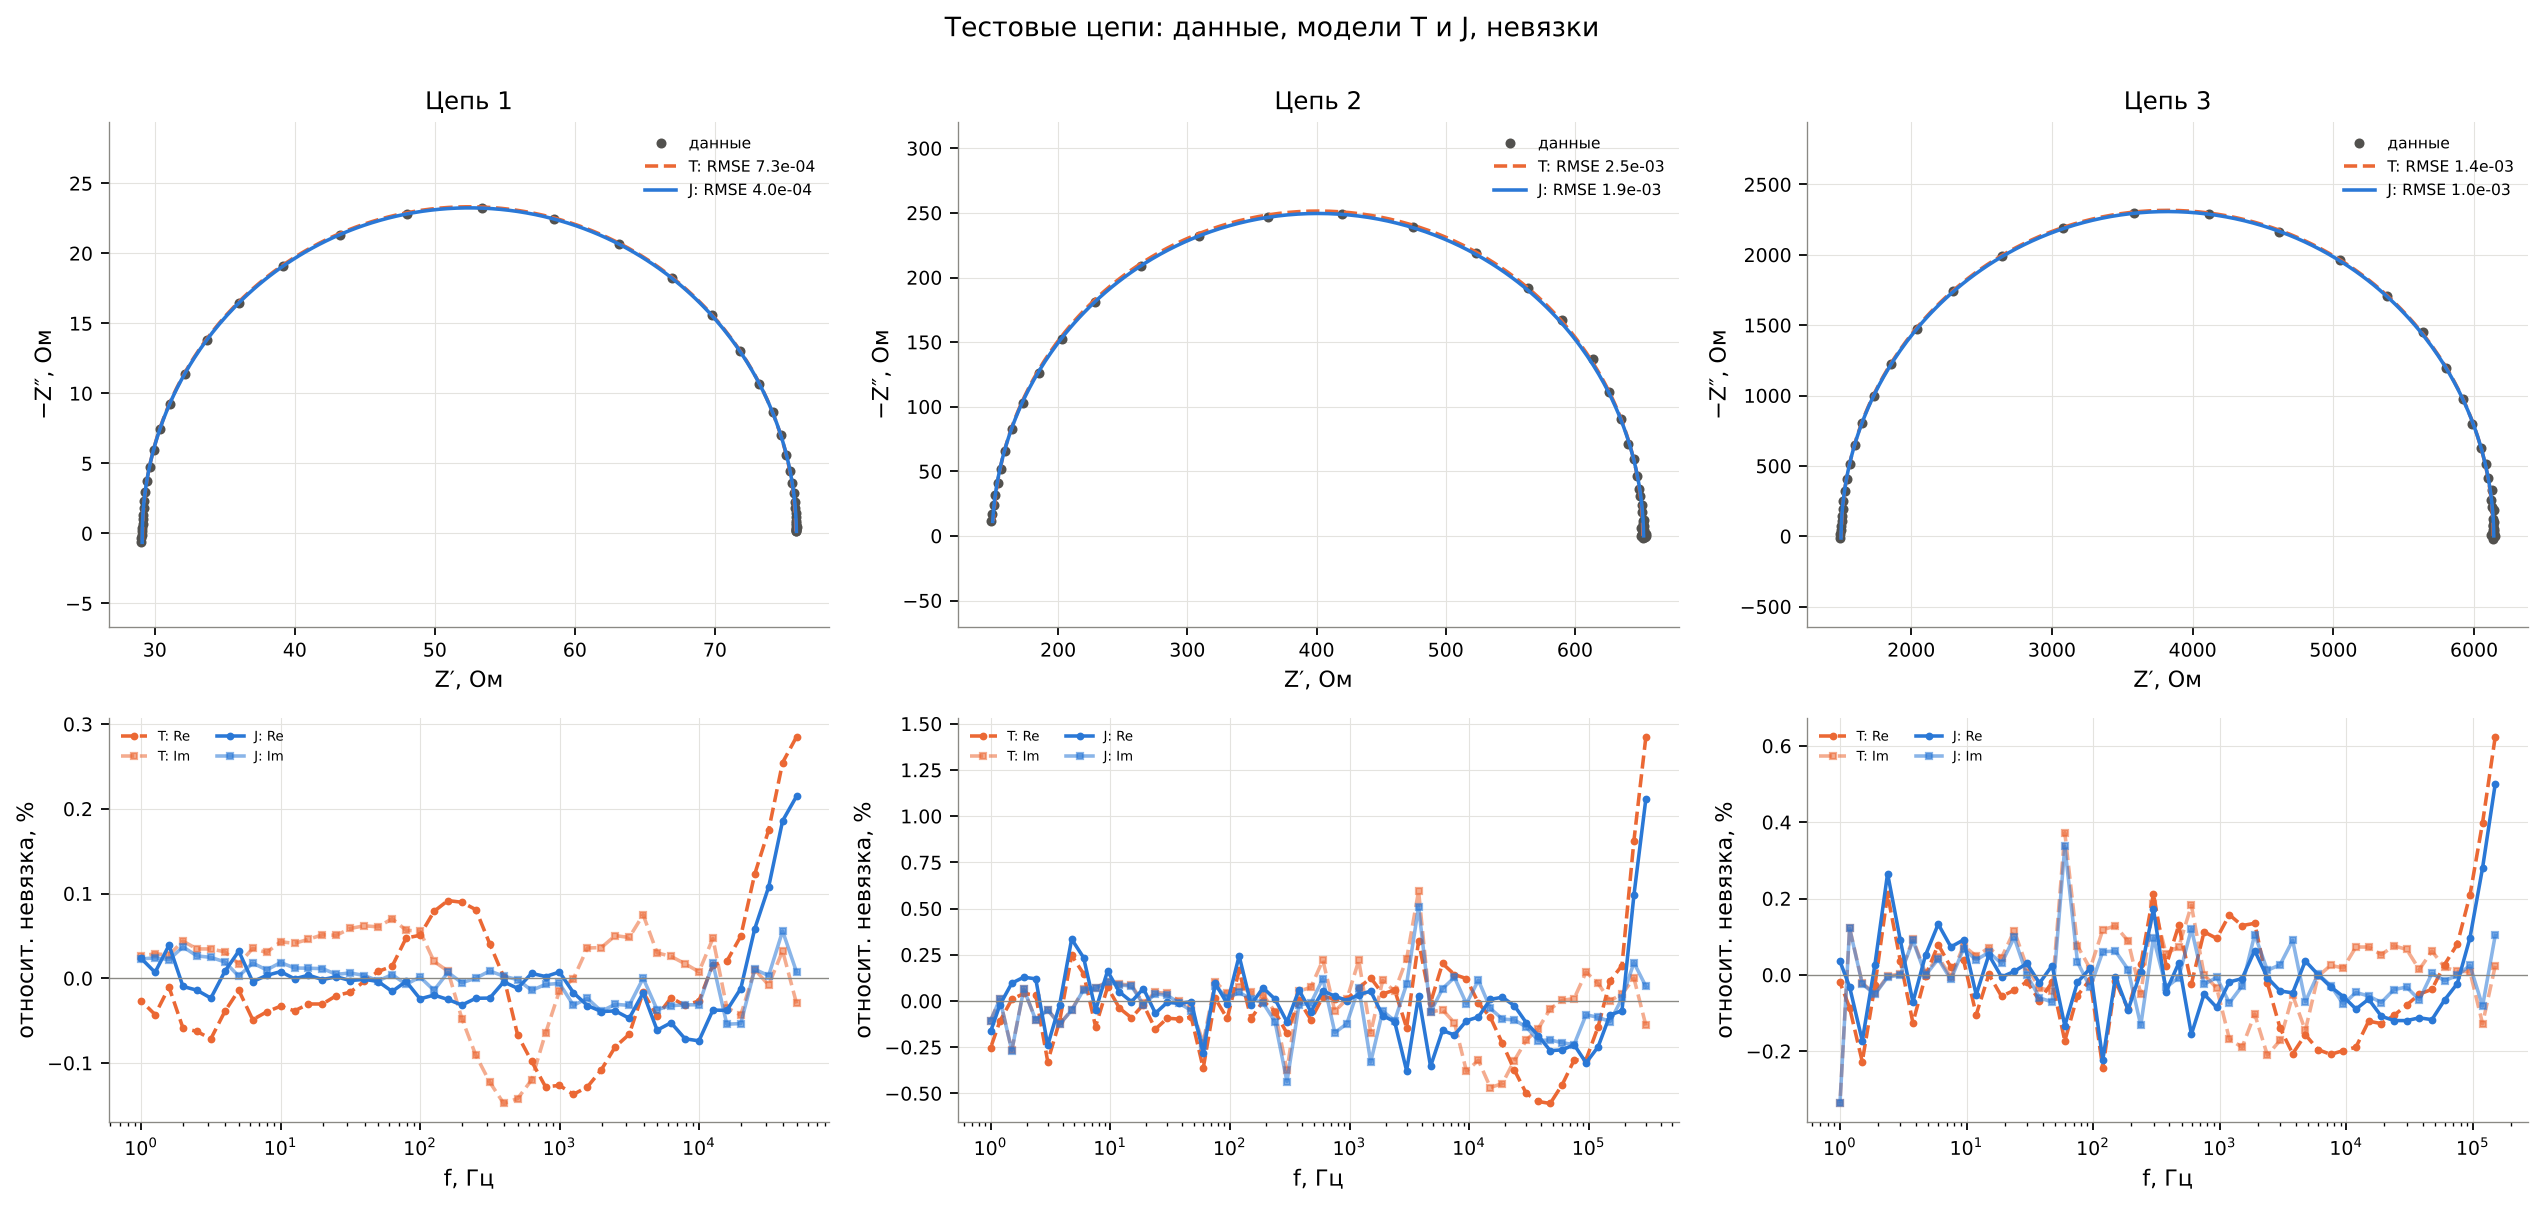
\includegraphics[width=0.86\linewidth]{fit_test_circuits.png}\\
  \small T: 0{,}07--0{,}25\,\%;\ J: 0{,}04--0{,}20\,\%, $\Delta$BIC $=-50\ldots-110$;\ $\hat\alpha=0{,}994$--$0{,}997$ (диэлектрическая абсорбция), $\hat\beta\to1$.
\end{frame}

\begin{frame}{Li-ion элемент: H2}
  \begin{columns}[T]
    \column{0.5\linewidth}
    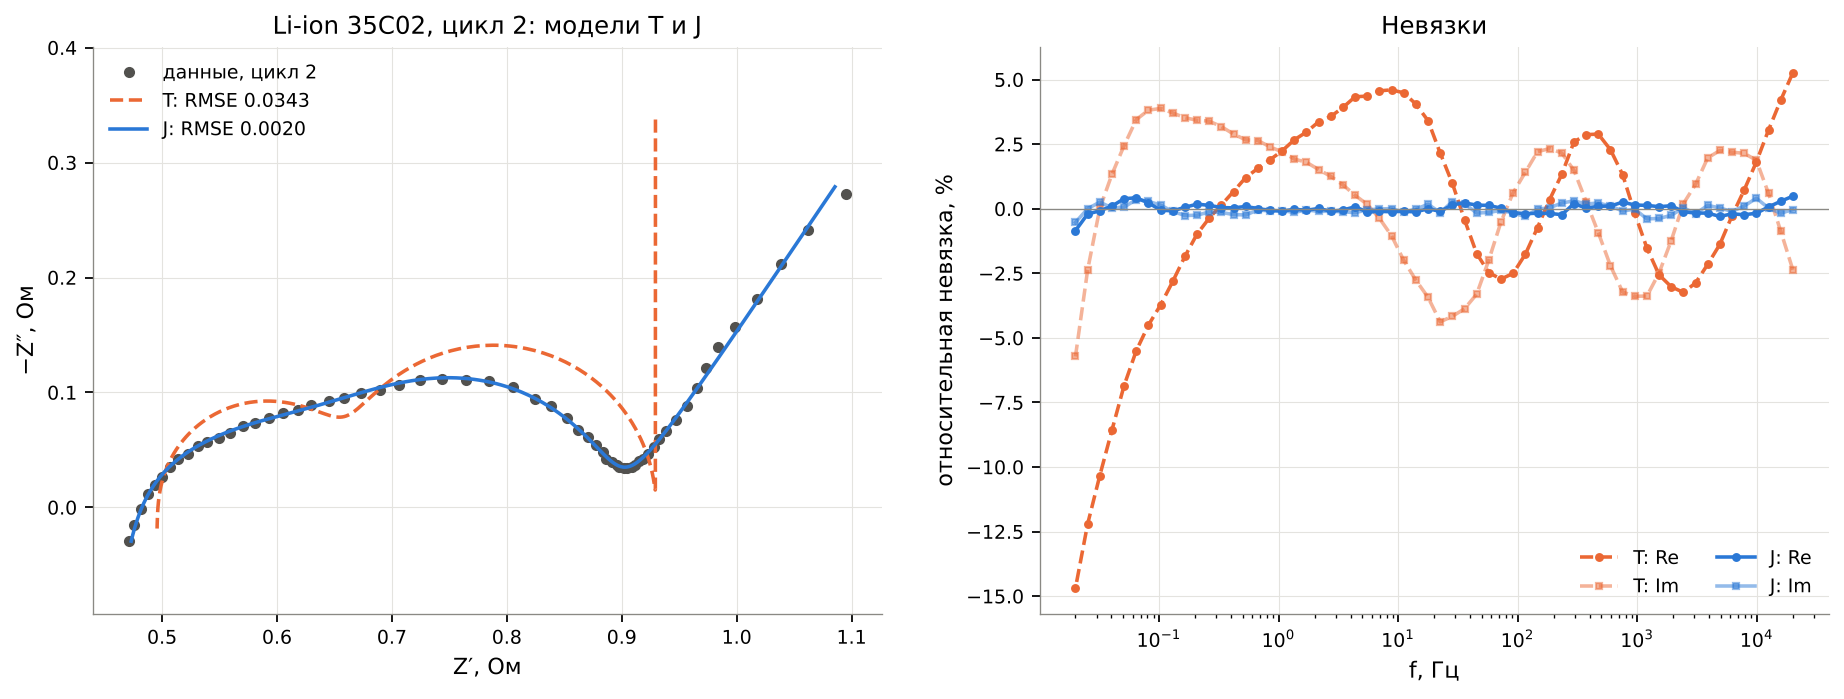
\includegraphics[width=\linewidth]{fit_battery_cycle2.png}\\
    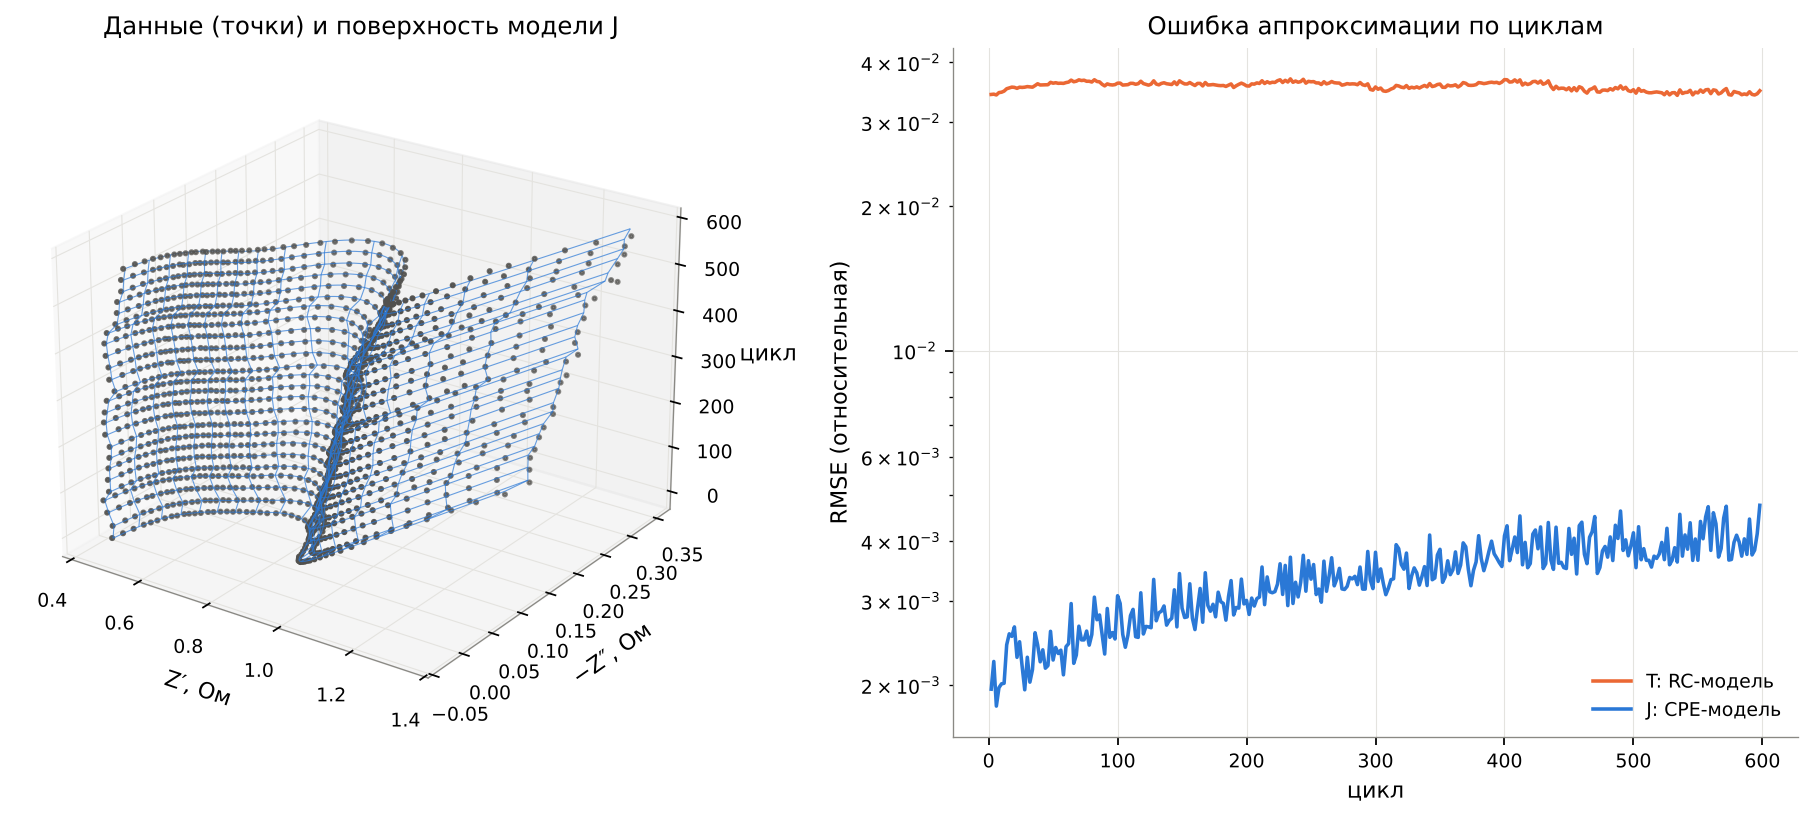
\includegraphics[width=\linewidth]{battery_fit_3d.png}
    \column{0.5\linewidth}
    \small
    \begin{itemize}
      \item T: RMSE 3{,}4--3{,}7\,\% со структурой невязок; J: 0{,}2--0{,}5\,\%; $\Delta$BIC $\approx-670$.
      \item 299 спектров: продолжение по циклам + контроль DE (выигрыш $<10^{-12}$).
      \item $R_2$: $0{,}17\to0{,}31$~Ом, $\rho(R_2,\text{ёмкость})=-0{,}99$.
      \item Дуги перекрываются: $\rho(R_1,R_2)=-0{,}99$; надёжна сумма $R_1+R_2$ (1--2.5\,\% против 7--13\,\%).
      \item Жадный поиск структуры по BIC: T $\xrightarrow{C_3\to Q_3}\xrightarrow{C_1\to Q_1}\xrightarrow{C_2\to Q_2}$ J через смешанные модели.
    \end{itemize}
  \end{columns}
\end{frame}

\begin{frame}{Траектории параметров}
  \centering
  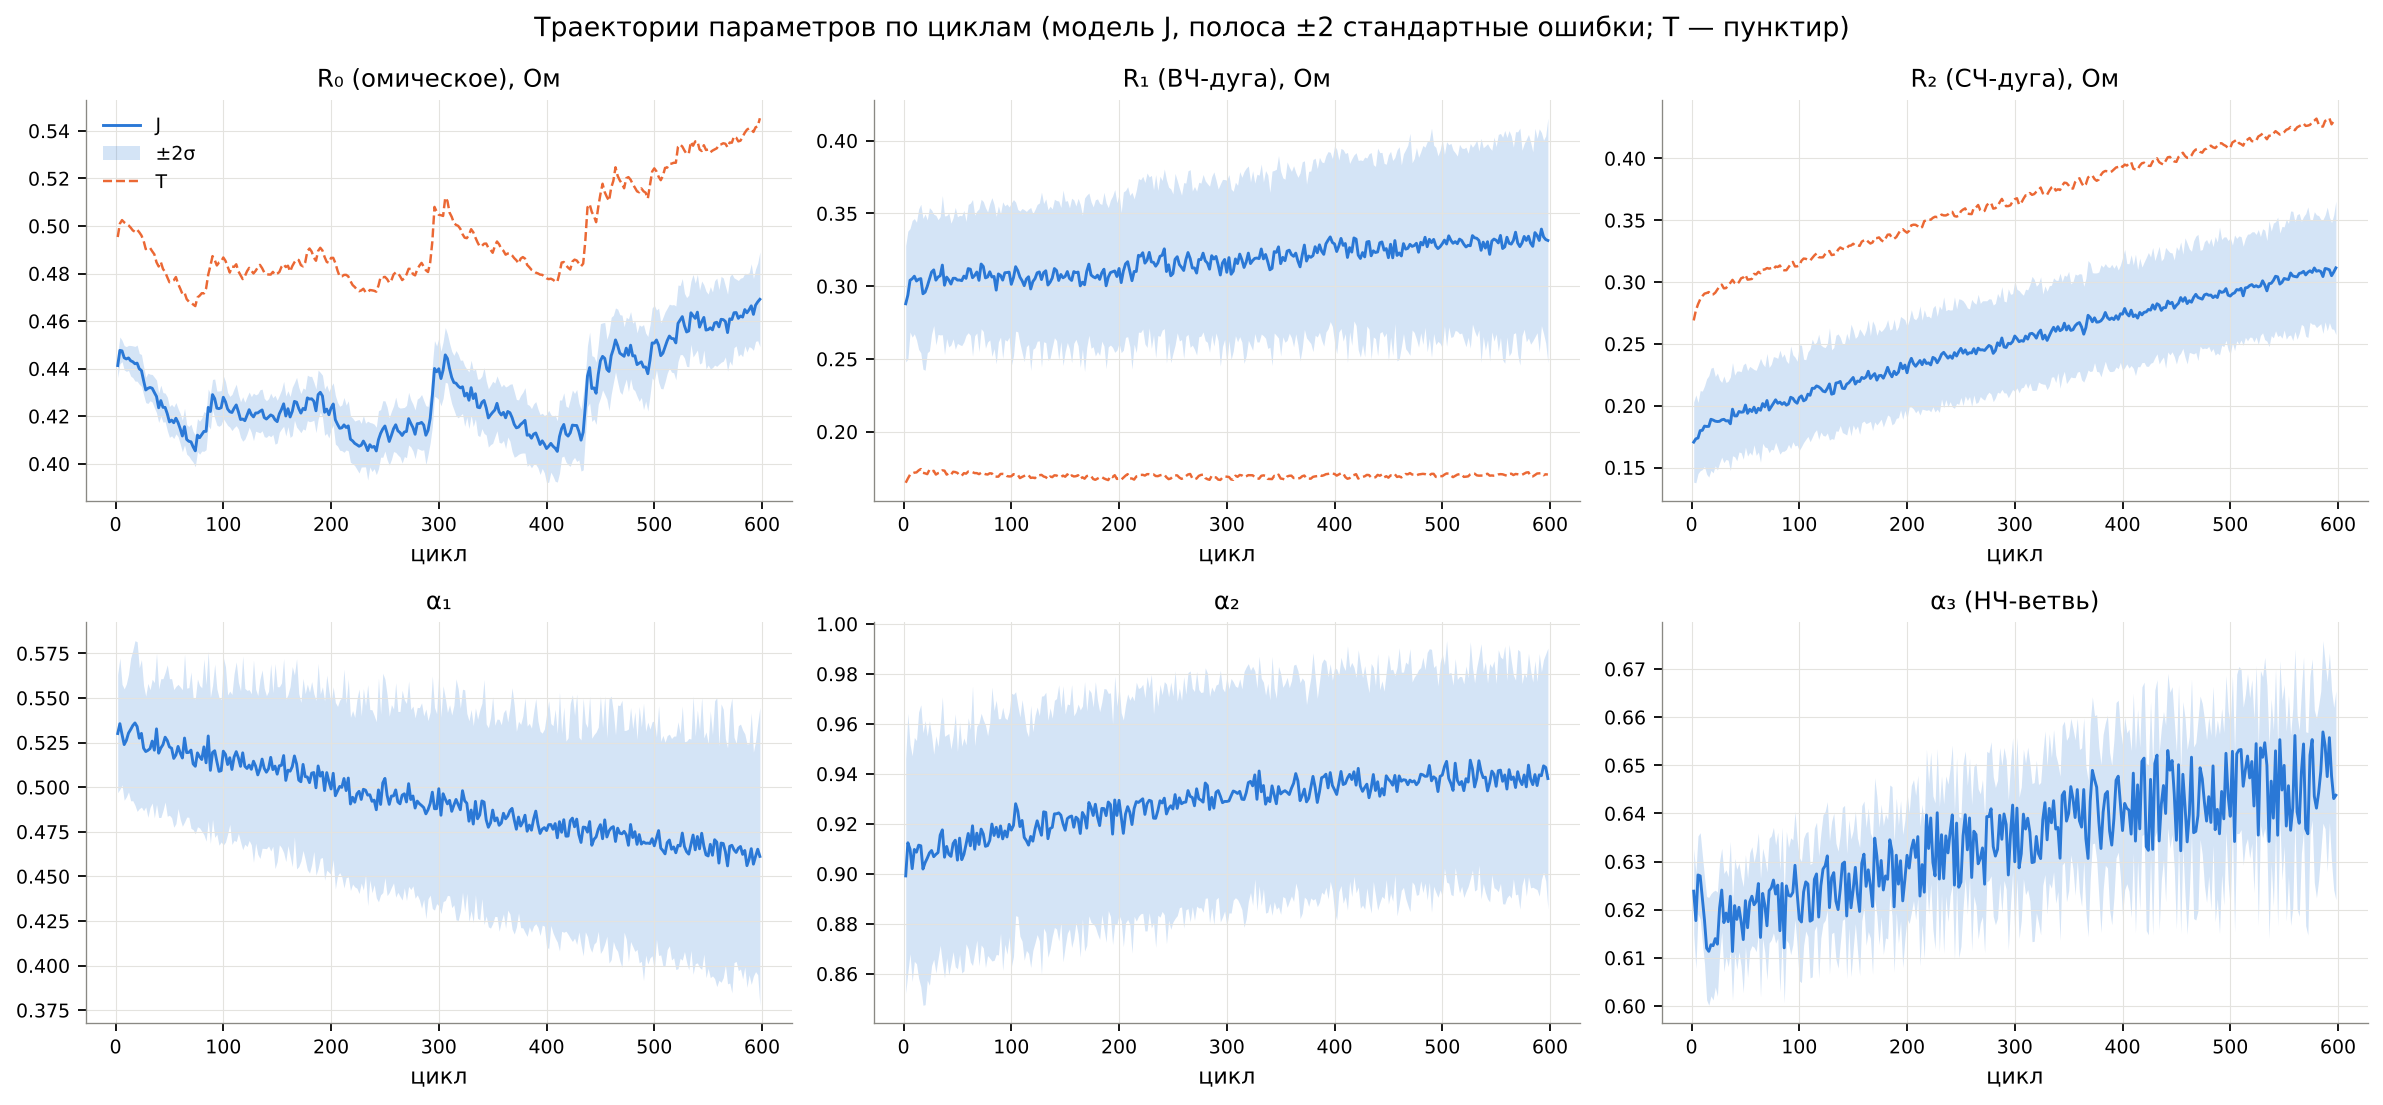
\includegraphics[width=0.92\linewidth]{battery_parameters.png}
\end{frame}

\begin{frame}{Резонаторы: H3}
  \centering
  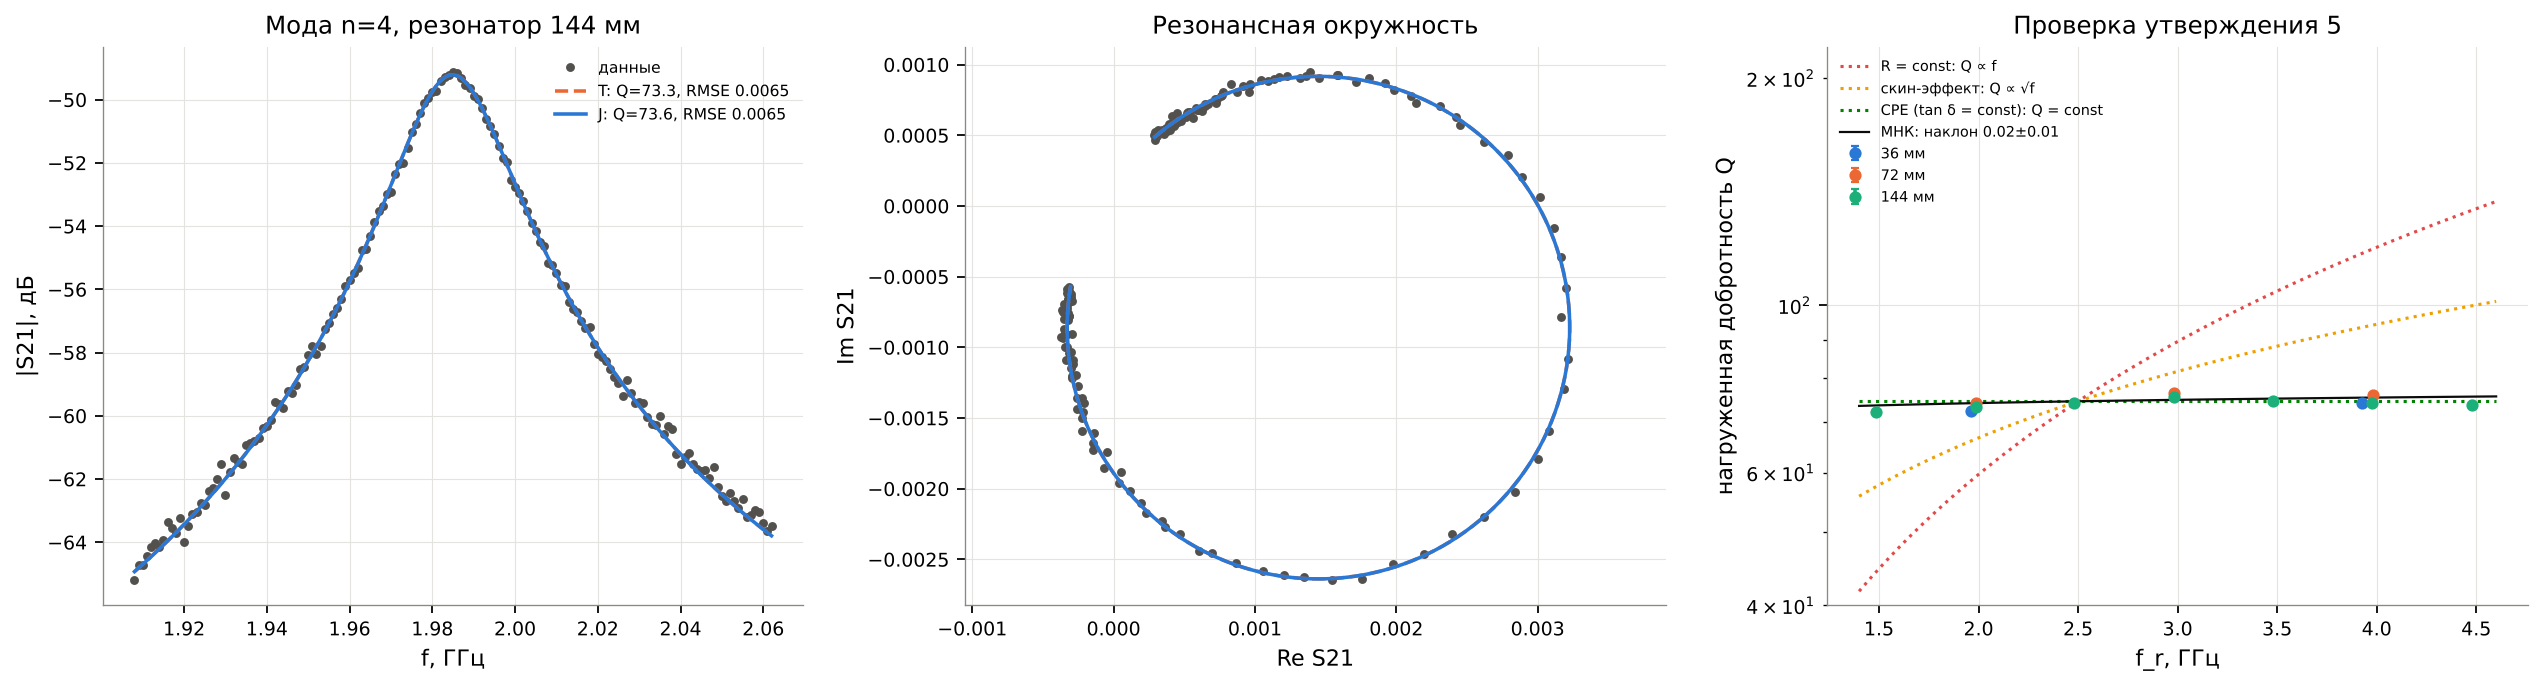
\includegraphics[width=\linewidth]{fit_resonators.png}\\
  \small По одной моде T и J неразличимы ($|\Delta\mathrm{BIC}|<1$); по 12 модам $d\ln Q/d\ln f=0{,}02\pm0{,}01$ $\Rightarrow$ CPE-диэлектрик,
  $\tan\delta_{\rm eff}\approx0{,}013$, $\varepsilon_{\rm eff}\approx4{,}4$.
\end{frame}

\begin{frame}{Временная область}
  \centering
  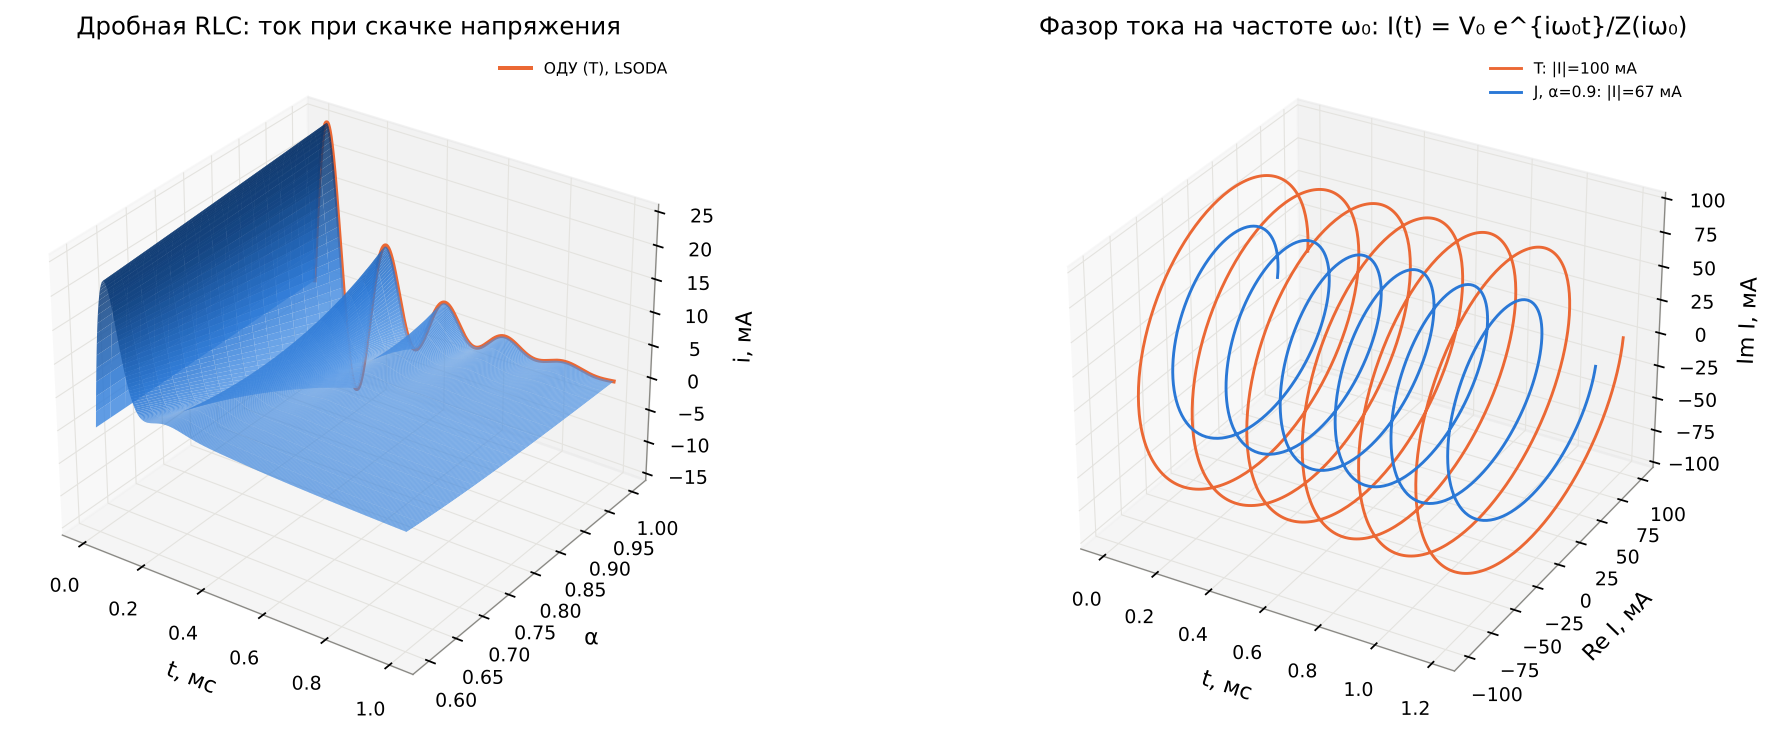
\includegraphics[height=0.4\textheight]{time_3d_rlc.png}\\
  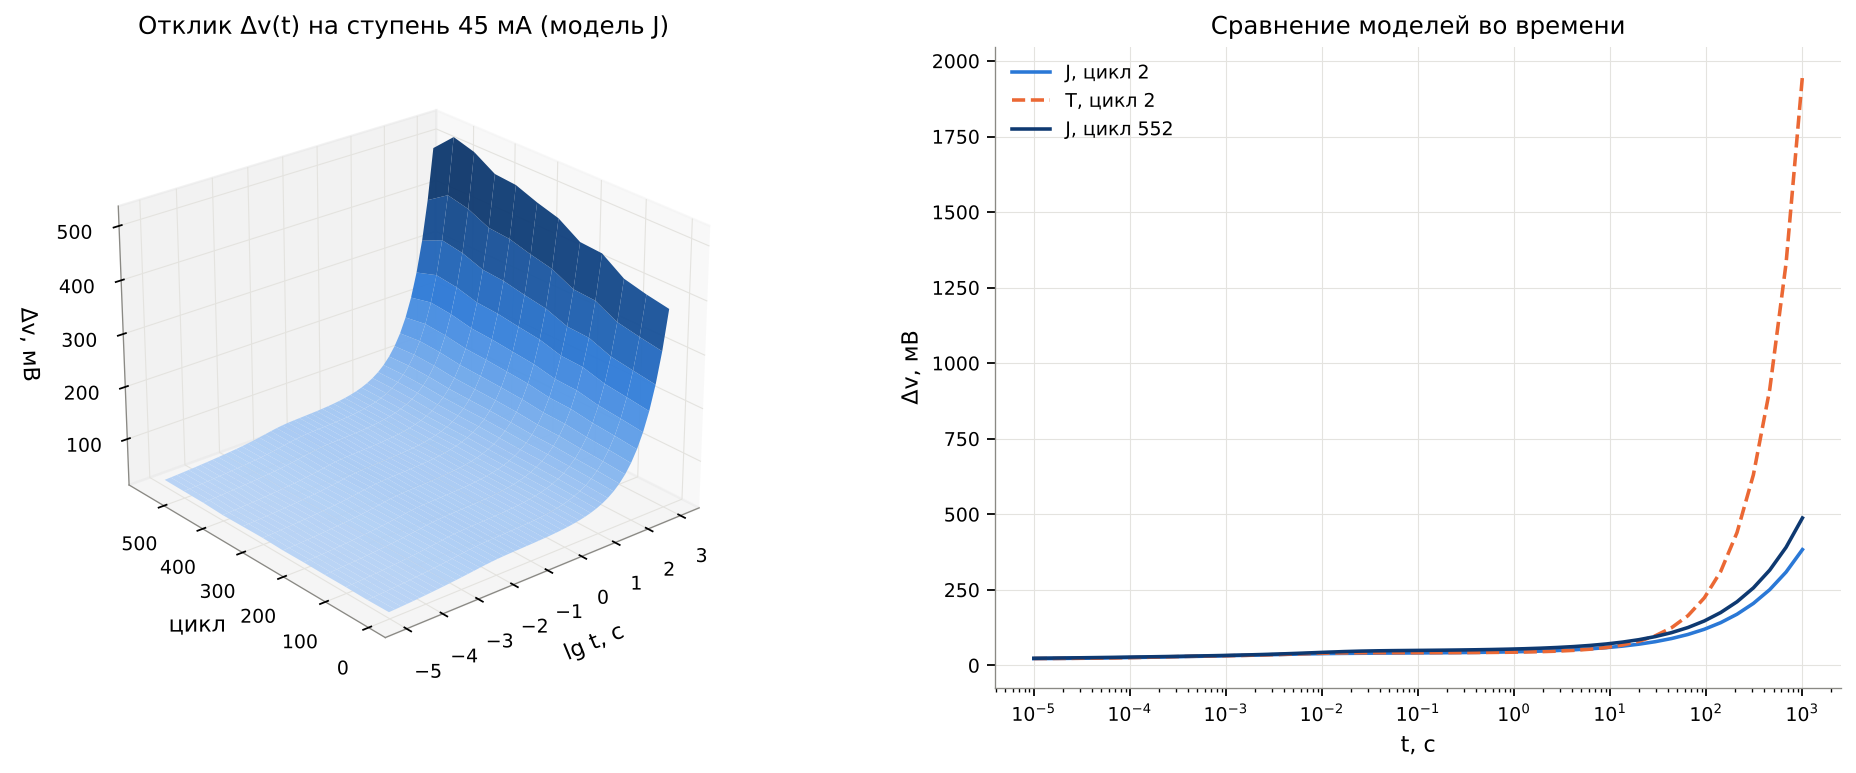
\includegraphics[height=0.4\textheight]{battery_time_3d.png}\\
  \footnotesize $i(t,\alpha)$: от учебной ($\alpha=1$, совпадает с LSODA) к дробной; фазор тока; $\Delta v(t,\text{цикл})$ батареи (Талбот).
\end{frame}

\begin{frame}{Выводы}
  \small
  \begin{enumerate}
    \item Учебная модель $\subset$ журнальной; доказаны пассивность, резонанс, $\tan\delta=\cot\frac{\alpha\pi}{2}$, закон $Q_n$, идентифицируемость до перестановок.
    \item Нужность дробного порядка определяется объектом \emph{и полосой данных}: малая, но значимая для конденсаторов; решающая для батареи; неразличима по одной моде, но видна по набору мод резонатора.
    \item Символьное представление окупается: точный якобиан, графы, проверки доказательств.
    \item Задел: \texttt{perturb.perturb\_data} (ЛР~2), \texttt{perturb.structural\_neighbours} и смешанные модели (ЛР~3).
  \end{enumerate}
  \medskip
  \textbf{Воспроизводимость:} \texttt{make all}; закреплённые коммиты, SHA-256, \texttt{seed=0}; 96 тестов.\\
  \textbf{ИИ:} весь репозиторий создан Claude Opus~5.5; промпт, скиллы и проверки~--- в \texttt{ai/AI\_USAGE.md}.
\end{frame}

\end{document}
